\begin{figure}[t]
\begin{minipage}[t]{0.166\textwidth}
\centering\textbf{\colorbox{white}{\scalebox{.8}{Ground-truth}}}
\end{minipage}\begin{minipage}[t]{0.166\textwidth}
\centering \textbf{\colorbox{white}{\scalebox{.8}{Standard}}}
\end{minipage}\begin{minipage}[t]{0.1725\textwidth}
\centering \textbf{\colorbox{white}{\scalebox{.8}{AR (Ours)}}}
\end{minipage}\begin{minipage}[t]{0.166\textwidth}
\centering\textbf{\colorbox{white}{\scalebox{.8}{Ground-truth}}}
\end{minipage}\begin{minipage}[t]{0.166\textwidth}
\centering \textbf{\colorbox{white}{\scalebox{.8}{Standard}}}
\end{minipage}\begin{minipage}[t]{0.166\textwidth}
\centering \textbf{\colorbox{white}{\scalebox{.8}{AR (Ours)}}}
\end{minipage}

\vspace{-0.1 cm}    
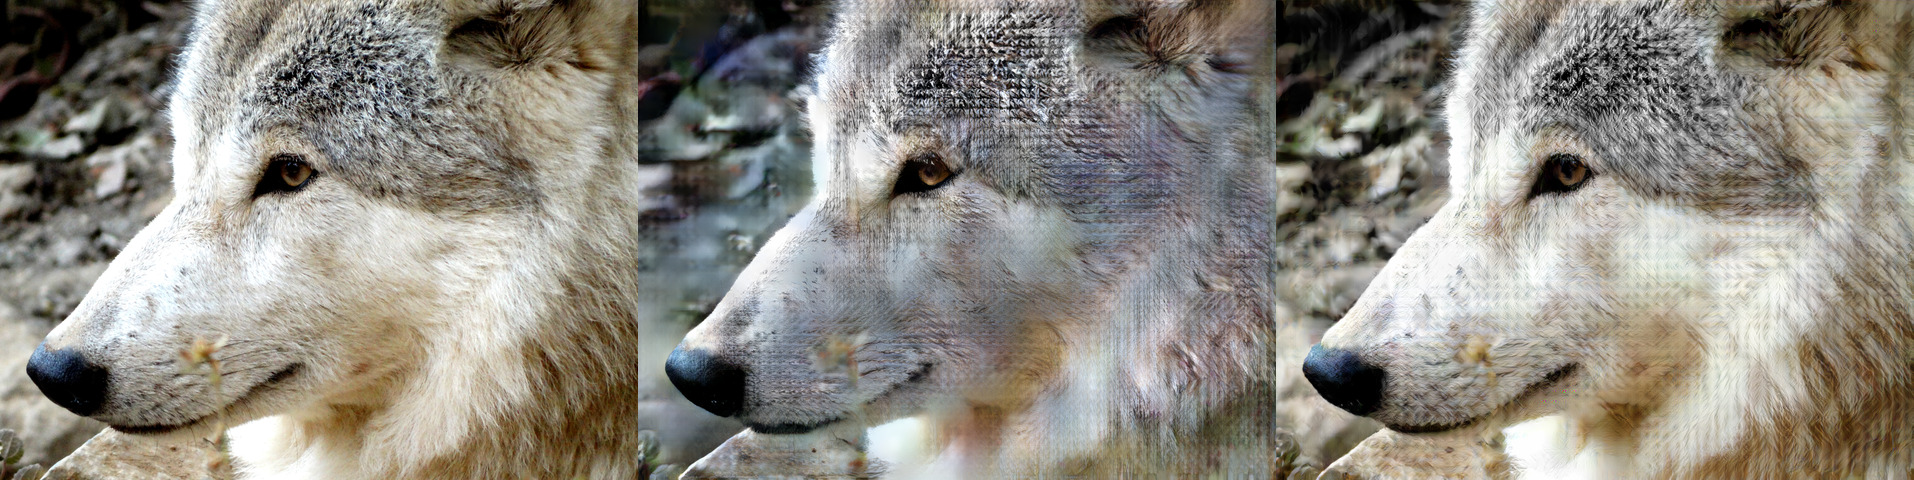
\includegraphics[width=0.5\textwidth]{figs/hires/tile_hires01_7.jpg}
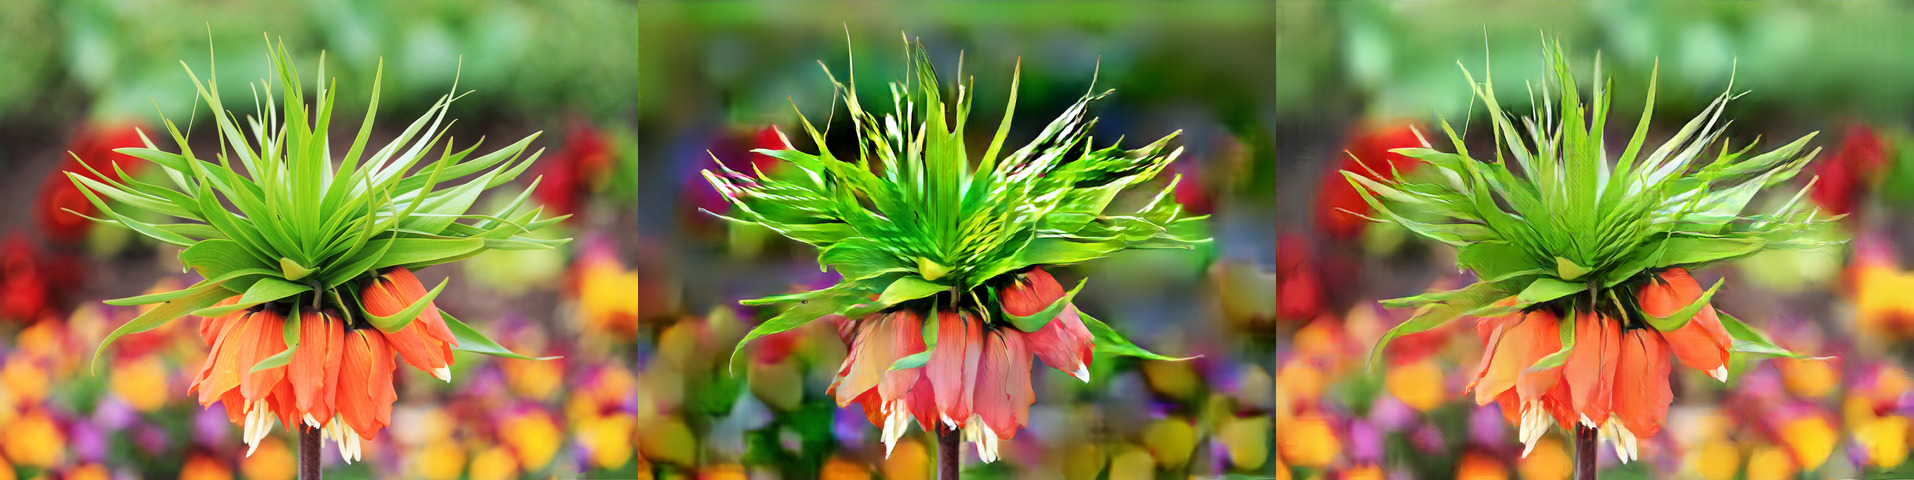
\includegraphics[width=0.5\textwidth]{figs/hires/tile_hires01_5.jpg}

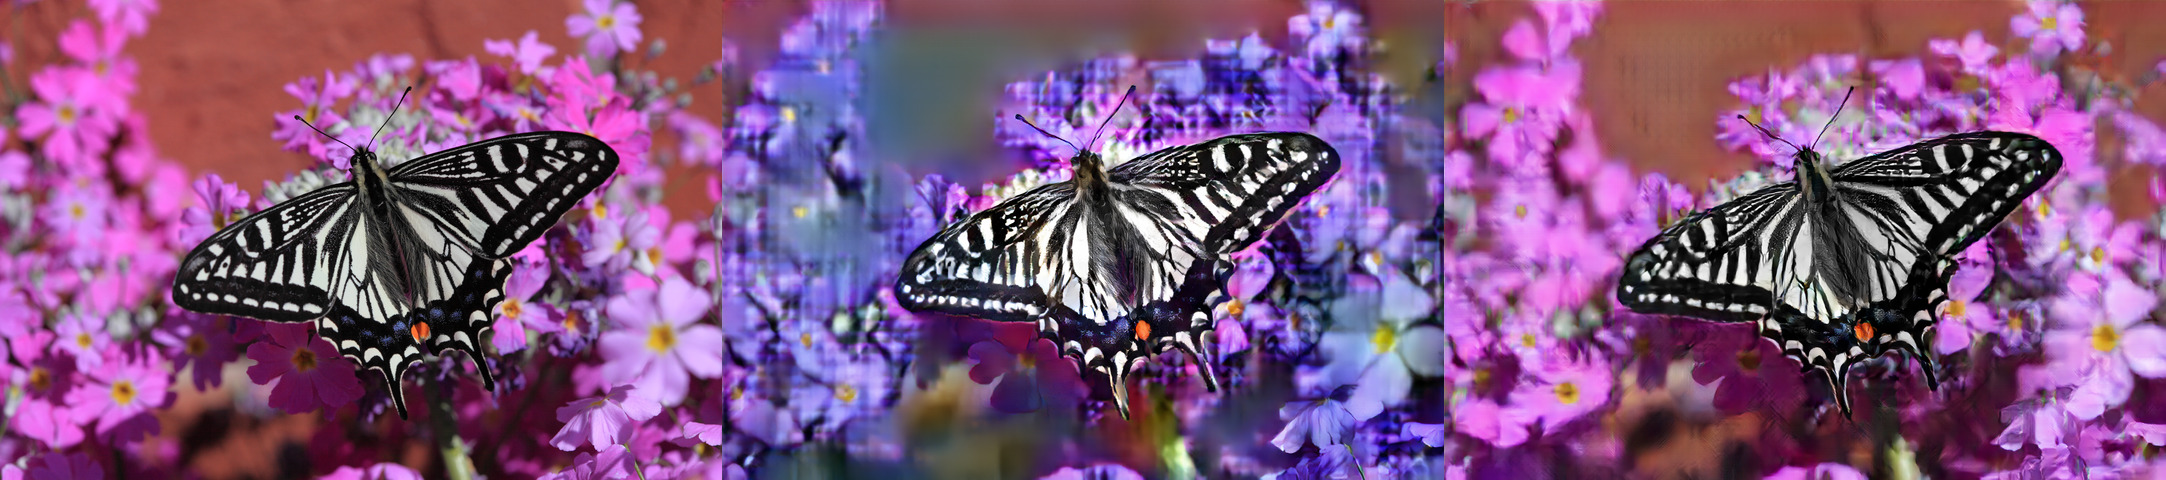
\includegraphics[width=0.5\textwidth]{figs/hires/tile_hires01_10.jpg}
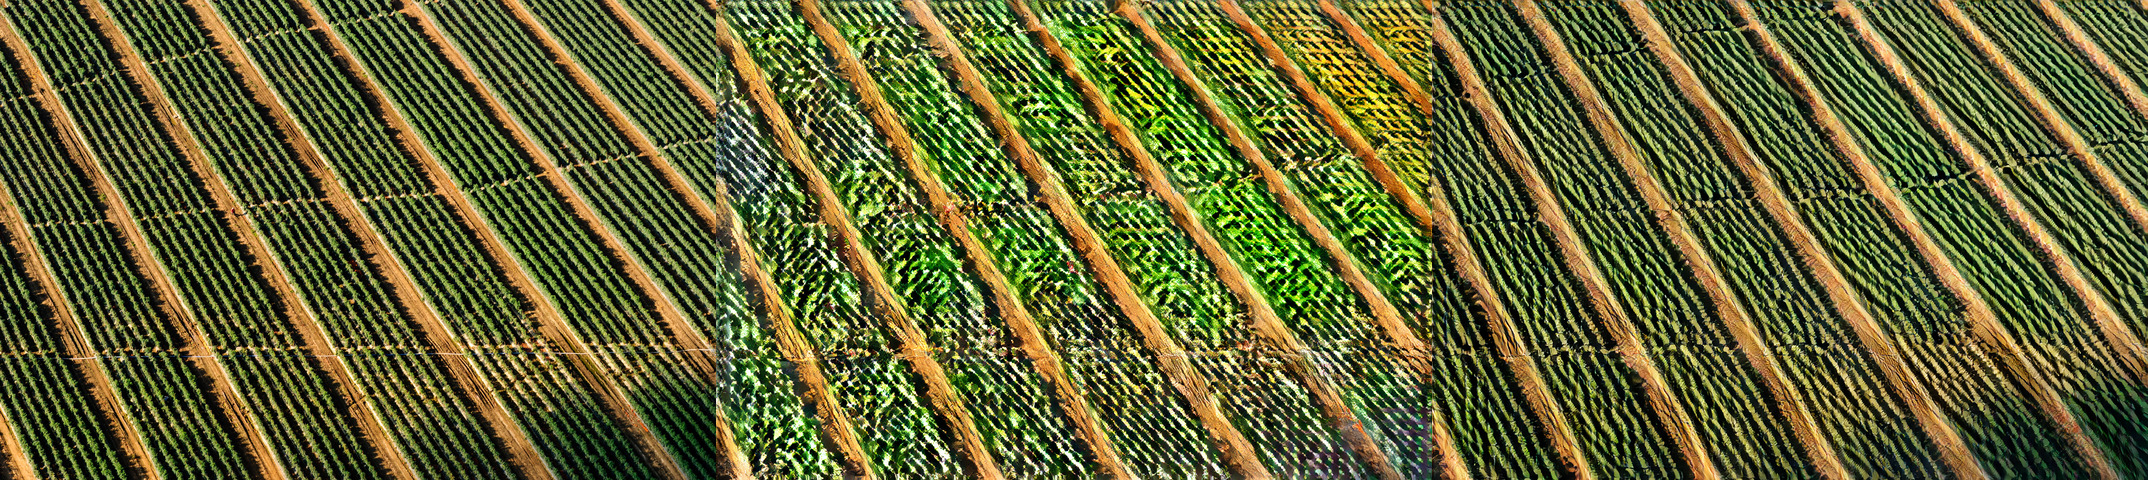
\includegraphics[width=0.5\textwidth]{figs/hires/tile_hires01_11.jpg}

\vspace{-0.1 cm}
\caption{\label{fig:hires}At a resolution of $2040\times 1536$ px., $10$ times larger than training samples, standard reconstructions on DIV2K show color and structure degradation. In contrast, reconstructions from our AR model do not suffer from distortions.}
\vspace{-0.5 cm}
\end{figure}
